% Format:  Latex Orientation:  Portrait
% MASTERFILE
%
% Last change: <Thu, 2016/05/26 10:25:26 arwagner l00slwagner.desy.de>
%
\documentclass[presentation, 10pt]{beamer}
% use ``handout'' instead of ``presentation'' to create a 2 on 1 page
% handout version of the document

\mode<handout>{%
	\usepackage{pgf}
	\usepackage{pgfpages}
	\pgfpagesuselayout{2 on 1}[a4paper,border shrink=5mm]
}
\mode<presentation>{%
	\usetheme{DESY}
}
%% Setup for Beamer
\usepackage{xcolor}
\usepackage{hyperxmp}
% \usepackage[pdfa]{hyperref}
\usepackage{luatextra}
\usepackage{wasysym}
\usepackage{eurosym}
\usepackage{bookmark}
\usepackage{graphicx}
\usepackage{fontspec}
\setmainfont{Arial}
\usepackage[ngerman,english]{babel}
\usepackage{xspace}
\usepackage{tikz}

\tikzset{%
  every overlay node/.style={%
    %draw=black,fill=white,rounded corners,anchor=north west,
    draw=fzjlightblue,fill=fzjgray30,rounded corners,anchor=north west,
  },
}
% Usage:
% \tikzoverlay at (-1cm,-5cm) {content};
% or
% \tikzoverlay[text width=5cm] at (-1cm,-5cm) {content};
\def\tikzoverlay{%
   \tikz[baseline,overlay]\node[every overlay node]
}%


% General new commands an macros
\renewcommand{\emph}[1]{\structure{#1}}

\newcommand{\link}[2]{\href{#1}{~#2}}

\newcommand{\jointwo}{\textbf{JOIN$^2$}\xspace}

\newcommand{\BibTeX}{Bib\TeX}
\newcommand{\JabRef}{\link{http://jabref.sf.net}{JabRef}\xspace}
\newcommand{\Companion}[1]{\textit{\link{http://julib.fz-juelich.de/uhtbin/field-search-sort/001/PBYR/213964}{\LaTeX{} Companion}, #1}\xspace}
\newcommand{\pkg}[1]{\emph{\texttt{#1}}\xspace}

% general colour definitions
\newcommand{\smallgray}[1]{{\tiny\emph{#1}}}

\newcommand{\idR}{i.~d.~R.\xspace}
\newcommand{\va}{v.~a.\xspace}
\newcommand{\sa}{s.~a.\xspace}
\newcommand{\zB}{z.~B.\xspace}
\newcommand{\zT}{z.~T.\xspace}
\newcommand{\ggf}{ggf.\xspace}
\newcommand{\eg}{e.~g.\xspace}

\newcommand{\bs}[1]{\texttt{$\backslash$#1}}
\newcommand{\command}[2]{\texttt{\bs{#1}\{#2\}}}
% http://tex.stackexchange.com/questions/16447/beamer-top-aligning-columns-within-a-top-aligned-fram
\makeatletter
\newenvironment{topitemize}{%
   \setlength{\topsep}{0pt}
   \setlength{\partopsep}{0pt}
   \renewcommand*{\@listi}{\leftmargin\leftmargini \parsep\z@ \topsep\z@ \itemsep\z@}
   \let\@listI\@listi
   \itemize
}{\enditemize}
\makeatother


\title{DQM4HEP \\ A data quality monitoring framework}
% subtitle is required for DESY beamer, set at least a space ~
\subtitle{BTTB6 2018 - Zurich}

\author[R. Ete]{\underline{R. Ete}, A. Pingault, T. Coates}
\institute{DESY}
\date{\today}

\newenvironment{topitemize}{%
   \setlength{\topsep}{0pt}
   \setlength{\partopsep}{0pt}
   \renewcommand*{\@listi}{\leftmargin\leftmargini \parsep\z@ \topsep\z@ \itemsep\z@}
   \let\@listI\@listi
   \itemize
}{\enditemize}

\usepackage{makecell}
\usepackage{pifont}

%---------------------------------------------------------------------

\begin{document}

\maketitle

%----------------------------------------------------------------------
\begin{frame}
  \frametitle{Summary}

  \begin{itemize}
    \item Introduction
    \item Framework presentation
    \item Experiments running with DQM4HEP
    \item Current status
    \item Ongoing and future work
  \end{itemize}
  
\end{frame}

% Detector  anomaly  detection:
% data taking is continuously monitored by physi-
% cists  taking  shifts  to  monitor  and  assess  the  quality  of  the  incoming  data,
% largely using reference histograms produced by experts.  A whole class of ML
% algorithms  called  anomaly  detection  can  be  useful  for  automating  this  im-
% portant task.  Such unsupervised algorithms are able to learn from data and
% produce an alert when deviations are observed.  By monitoring many variables
% at the same time, such algorithms are sensitive to subtle signs forewarning of
% imminent failure,  so that pre-emptive maintenance can be scheduled.  These
% techniques are already used in industry.

%----------------------------------------------------------------------
\begin{frame}
  \frametitle{DQM systems in a nutshell}
  \footnotesize
  
  \underline{DQM systems in HEP domain:}
  \begin{itemize}
    \item Automated data quality assessement 
    \item Alert users when anomalies are observed
    \item Provide for online/offline analysis 
    \begin{itemize}
      \scriptsize
      \item Automatic data quality tests, possibly with reference histograms
      \item Distributed system for online analysis (data collectors)
      \item Dedicated visualization interfaces for shifters
    \end{itemize}
    \item Must be \underline{scalable}: from prototypes to collider-like detectors
  \end{itemize}
  ~\\
  \underline{General goal of using a DQM framework in testbeams:}
  \begin{itemize}
    \scriptsize
    \item Having a better understanding of your DUT
    \item Understand your setup and run settings
    \item Avoid starting bad runs
    \item Discard bad/unexpected data
  \end{itemize}

\end{frame}




%----------------------------------------------------------------------
\begin{frame}
  \frametitle{DQM systems for testbeams}
  \footnotesize
  \underline{Typical use cases:}
  \begin{itemize}
    \pause
    \item Environmental/slow control monitoring
    \begin{itemize}
      \scriptsize
      \item Gas flow ? Current/HV ? Temperature ? Pressure ? B field ? \\
      $\rightarrow$ Avoid to start bad runs, discard bad runs
    \end{itemize}
    \pause
    \item Hit maps (e.g calorimeters or trackers)
    \begin{itemize}
      \scriptsize
      \item Detect inefficient areas \\
      $\rightarrow$ Discard bad data, understand your DUT
    \end{itemize}
    \pause
    \item Beam structure analysis
    \begin{itemize}
      \scriptsize
      \item Check particle properties: type, momentum/energy ... \\
      $\rightarrow$ Avoid starting bad runs
    \end{itemize}
    \pause
    \item Combine telescope + DUT
    \begin{itemize}
      \scriptsize
      \item Run tracking algorithm, quickly detect mis-alignment \\
      $\rightarrow$ Understand your setup, discard unexpected data 
    \end{itemize}
  \end{itemize}
  ~\\
  \pause
  \underline{Problem:} One experiment = one EDM = one framework !

  \begin{itemize}
    \item Detector algorithm (DA) \textcolor{red}{not re-usable} by other experiments
    \item Leads to \textcolor{red}{duplicated} software and efforts
    \item EDM dependency: custom prototype EDM make use of these framework complicated $\rightarrow$ Each new prototype comes with its \textcolor{red}{ad-hoc solution}
  \end{itemize}
  \pause
  \begin{center} \underline{Need for a more generic framework} \end{center}
  % Development of a generic DQM software for any HEP experiment : \textbf{DQM4HEP}

\end{frame}




%----------------------------------------------------------------------
\begin{frame}
  \frametitle{DQM4HEP}
  \framesubtitle{\textbf{D}ata \textbf{Q}uality \textbf{M}onitoring for \textbf{H}igh \textbf{E}nergy \textbf{P}hysics}
  \footnotesize
  \underline{Philosophy:}
  \begin{itemize}
    \item Encapsulate changes in (abstract) interfaces
    \begin{itemize}
      \scriptsize
      \item No EDM, just a handler for your data
      \item Data streaming: how should we read/write your data 
    \end{itemize}
    \item Make user code \textit{plugable}
    \begin{itemize}
      \scriptsize
      \item Plugins in shared library: plug and play
      \item Make the easily extensible
    \end{itemize}
    \item Framework based on these two features 
  \end{itemize}
  ~\\
  \underline{Features:}
  \begin{itemize}
    \item Core:
    \begin{itemize}
      \scriptsize
      \item Streaming tools for reading/writing event
      \item Quality test tools : interface + many templates
    \end{itemize}
    \item Online:
    \begin{itemize}
      \scriptsize
      \item Online analysis plugin (API)
      \item Distributed system (TCP/IP)
      \item Data collectors : event and histogram collector servers
      \item Remote process management
    \end{itemize}
  \end{itemize}

\end{frame}


%----------------------------------------------------------------------
\begin{frame}
  \frametitle{DQM4HEP}
  \framesubtitle{Quality test API}
  \footnotesize
  \begin{block}{\footnotesize Monitor element}
    \begin{itemize}
      \item Wrap a ROOT TObject 
      \item Optionally hold a ROOT TObject as reference
    \end{itemize}
  \end{block}
  \begin{block}{\footnotesize Quality test}
    \begin{itemize}
      \item Implement the logic for monitor element testing
      \item Output a quality report (quality flag, success, etc)
    \end{itemize}
  \end{block}
  \pause
  \underline{Concrete example:} \\
  \begin{minipage}{0.38\linewidth}
    \begin{itemize}
      \scriptsize
      \item $\pi^+$ beam in a calorimeter
      \item Plot the total energy distribution. %Assess if the mean energy value, using a gaussian fit, is within your expectations.
      \item Assess quality :
      \begin{itemize}
        \scriptsize
        \item Fit distribution with gaussian function
        \item Extract $\chi^2$ and mean value
        \item Check for any deviation
      \end{itemize}
    \end{itemize}
  \end{minipage}
  \begin{minipage}{0.3\linewidth}
    \centering
    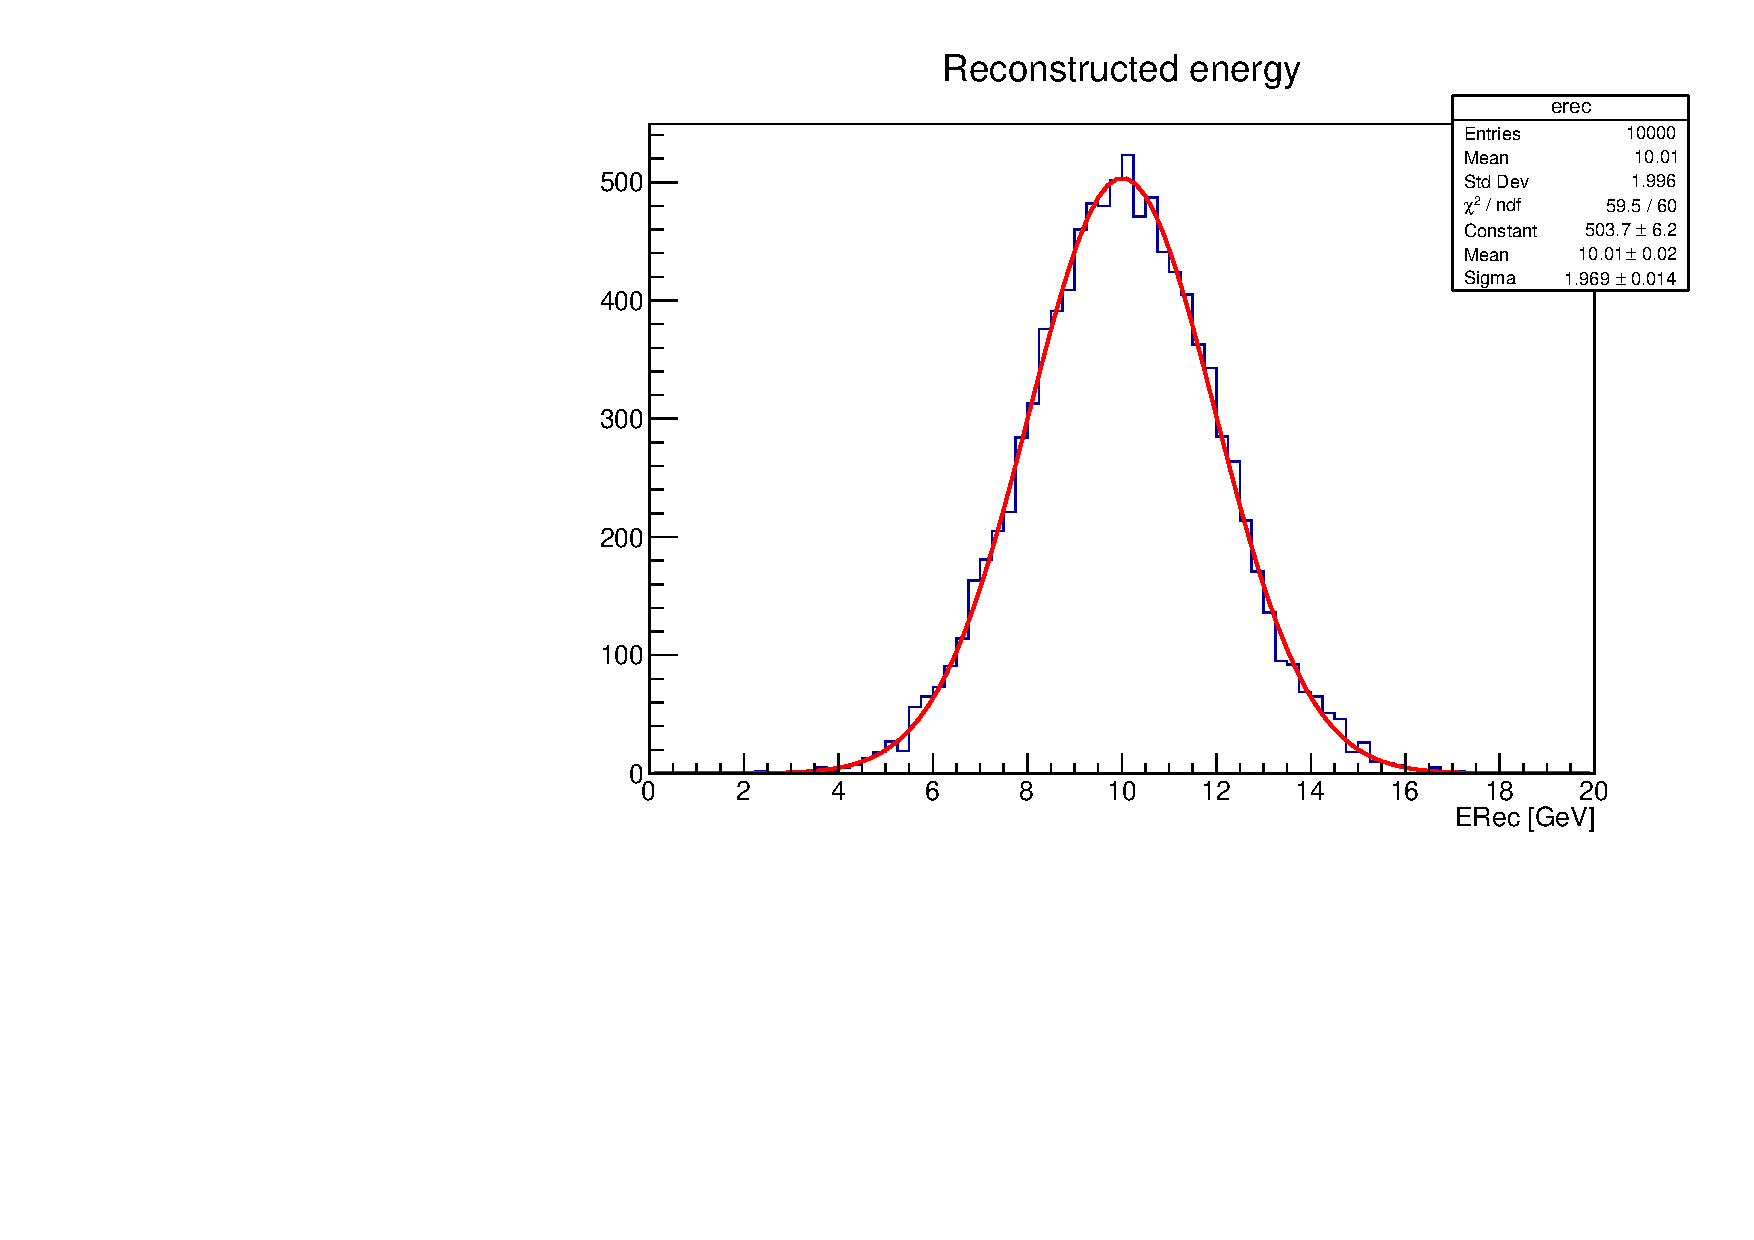
\includegraphics[width=\linewidth]{figs/ERecExample.pdf} \\
    Normal run
  \end{minipage}
  \begin{minipage}{0.3\linewidth}
    \centering
    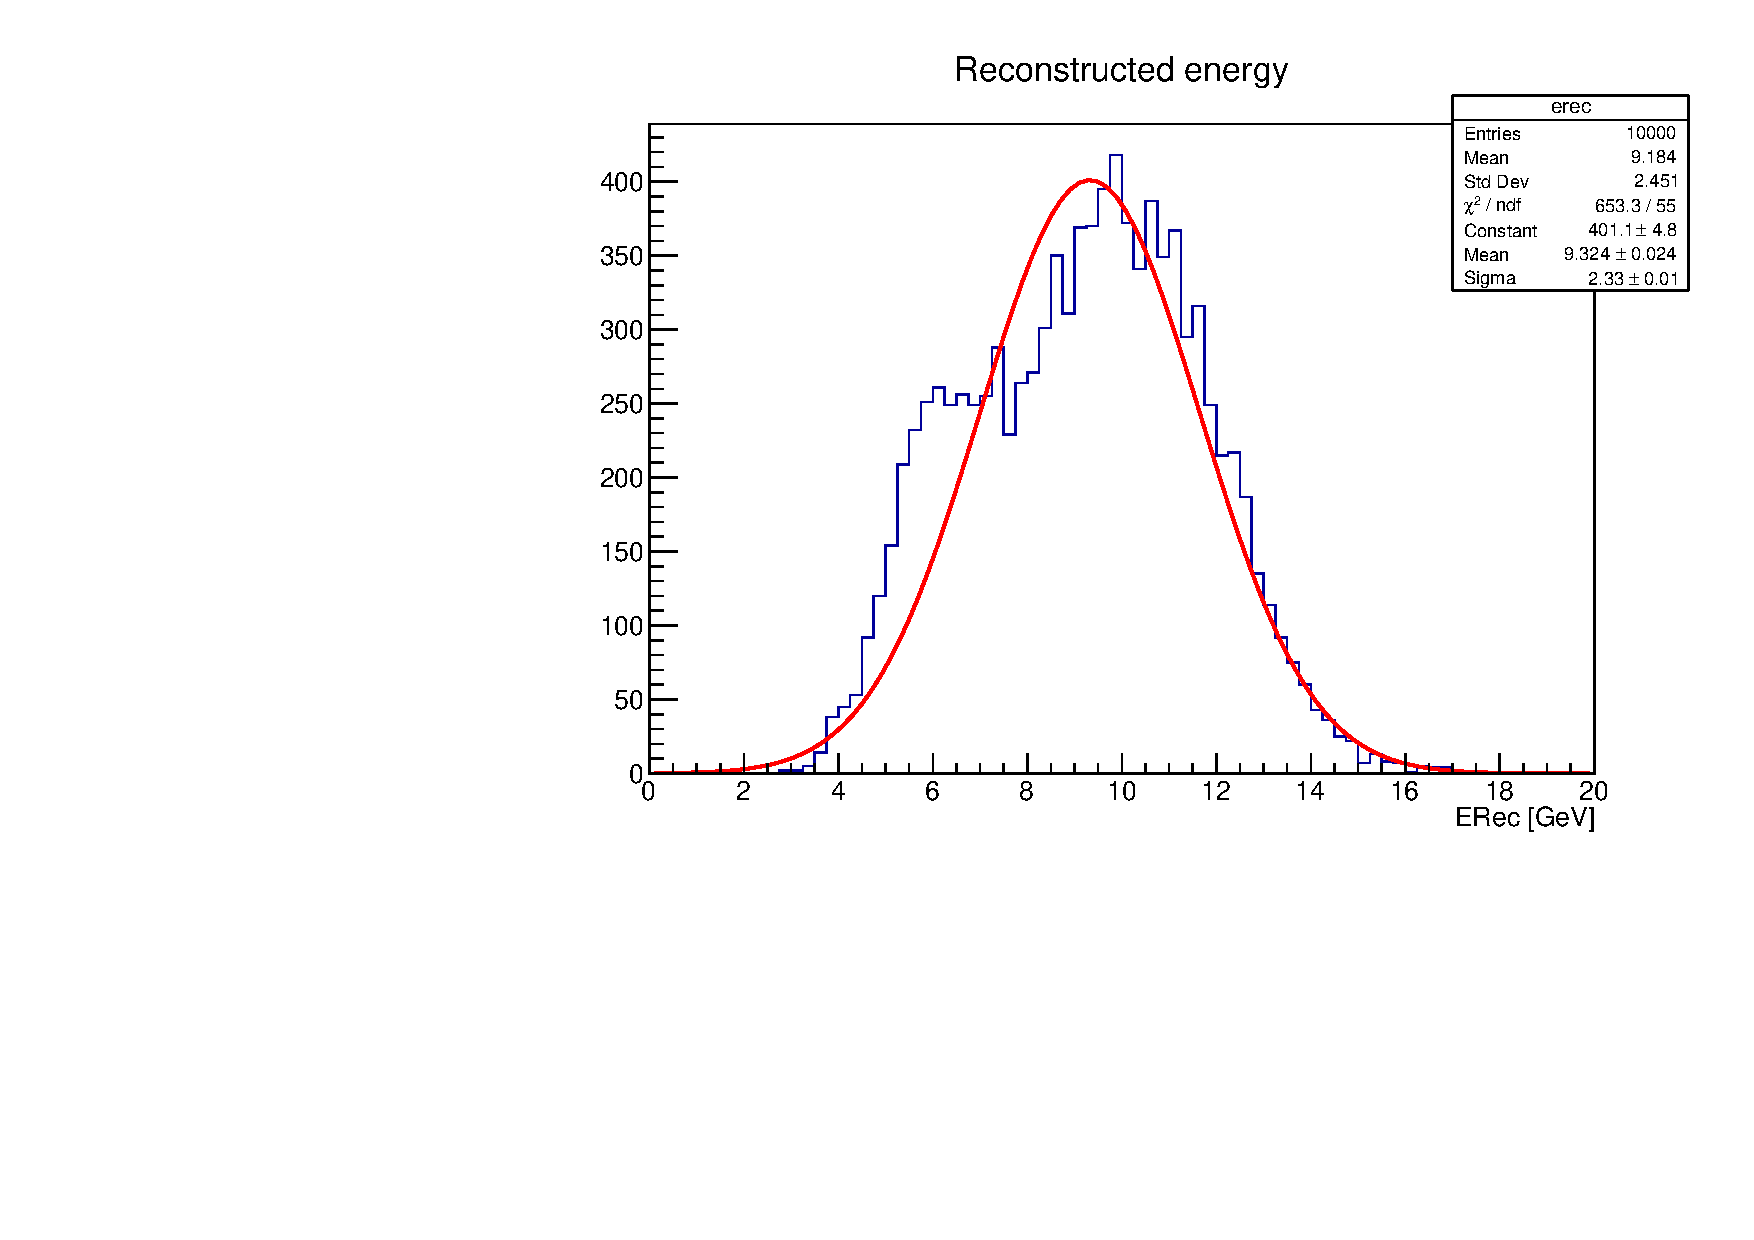
\includegraphics[width=\linewidth]{figs/ERecExampleUnexpected.pdf} \\
    Beam conversion ?
  \end{minipage}
\end{frame}

%----------------------------------------------------------------------
\begin{frame}
  \frametitle{DQM4HEP}
  \framesubtitle{Online architecture}
  \centering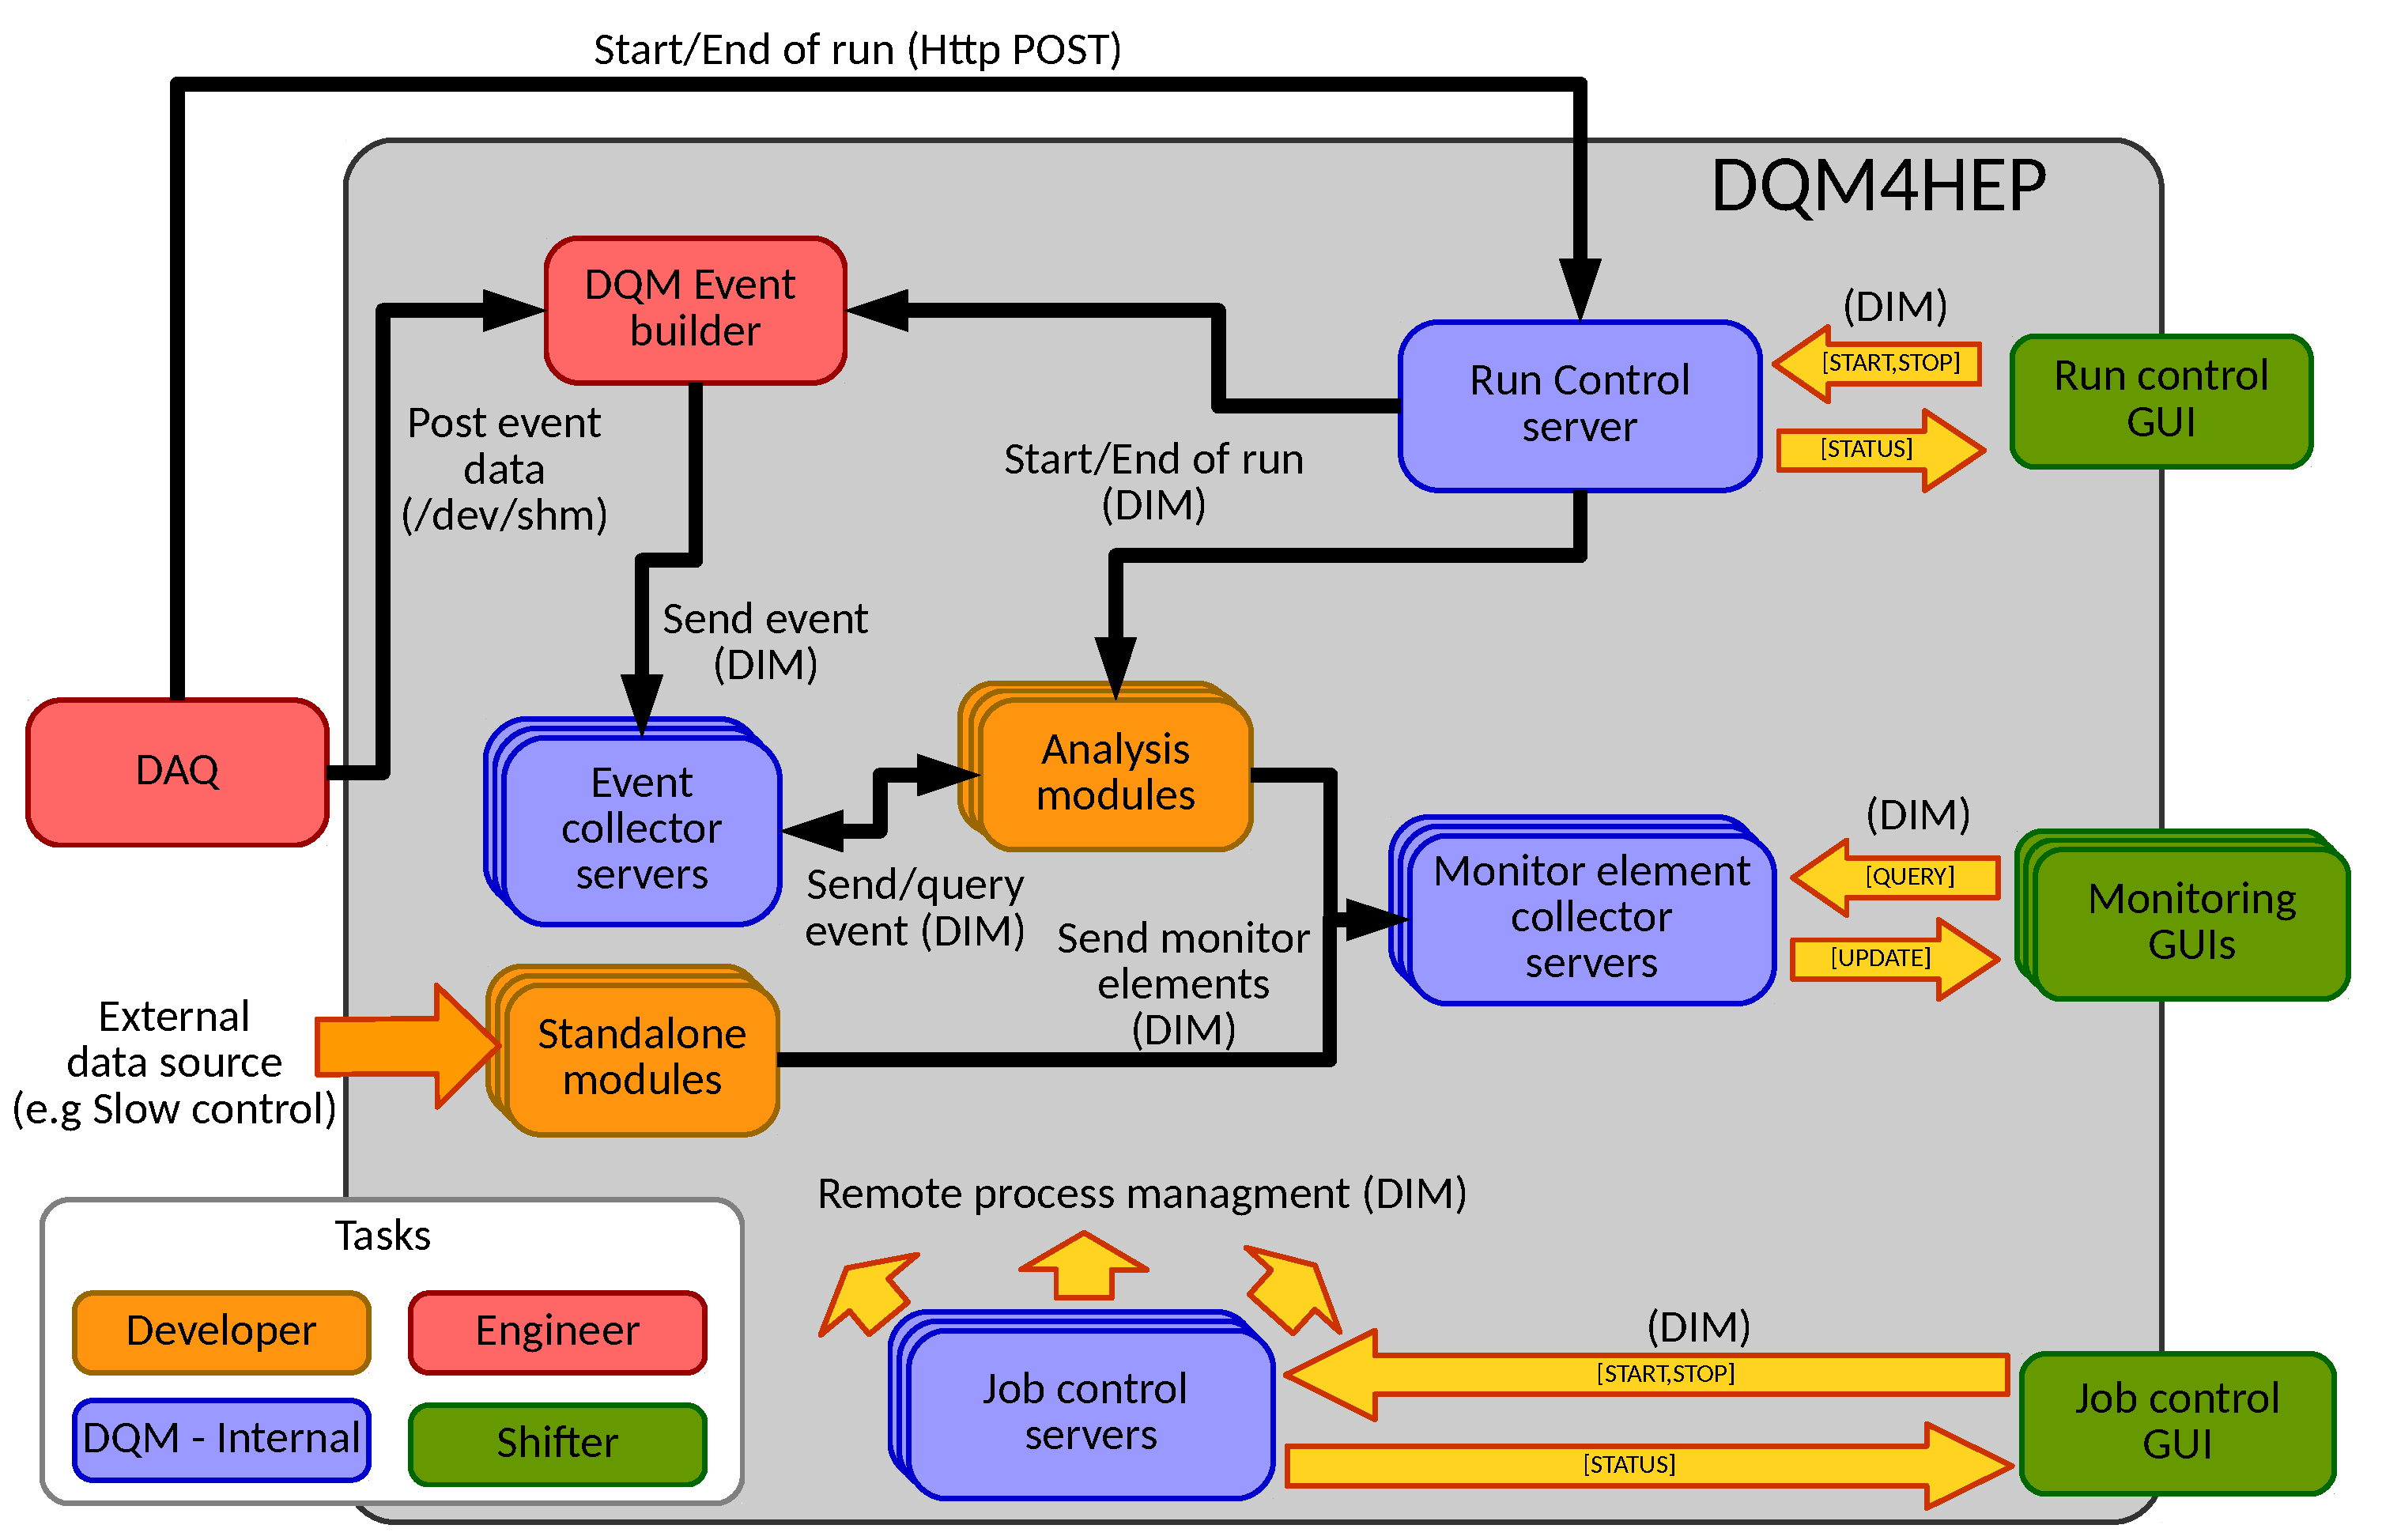
\includegraphics[width=0.9\linewidth]{figs/GlobalArchitectureDiagram.pdf}
\end{frame}

%----------------------------------------------------------------------
\begin{frame}
  \frametitle{DQM4HEP}
  \framesubtitle{Data analysis module}
  \centering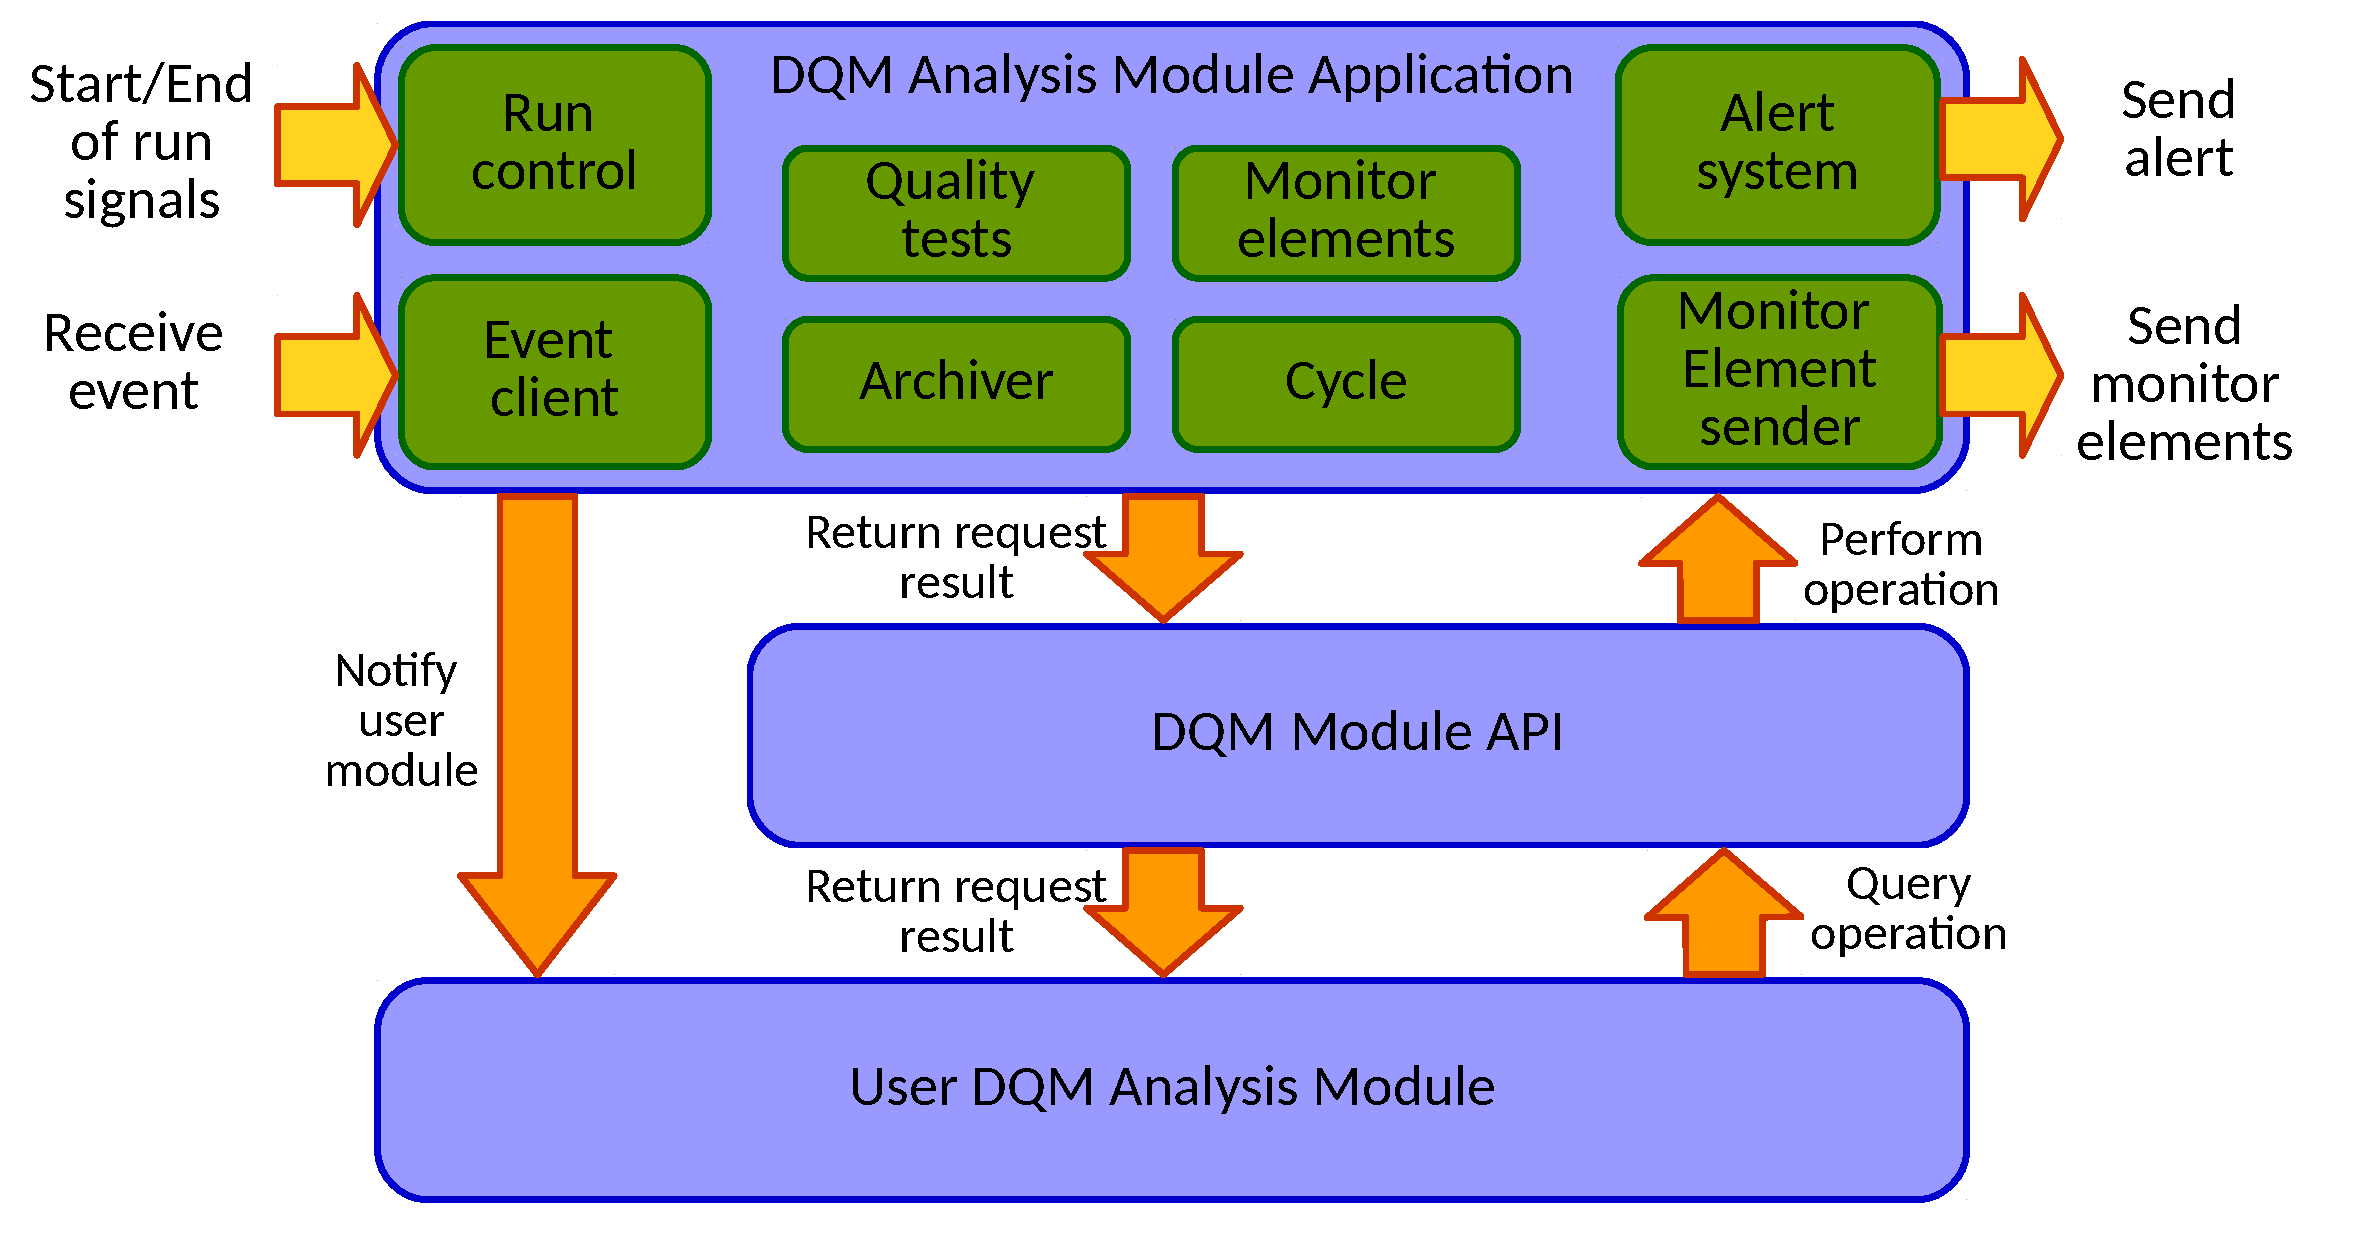
\includegraphics[width=0.9\linewidth]{figs/AnalysisModuleApplicationDiagram.pdf}
\end{frame}

%----------------------------------------------------------------------
\begin{frame}
  \frametitle{DQM4HEP}
  \framesubtitle{Slow control module}
  \centering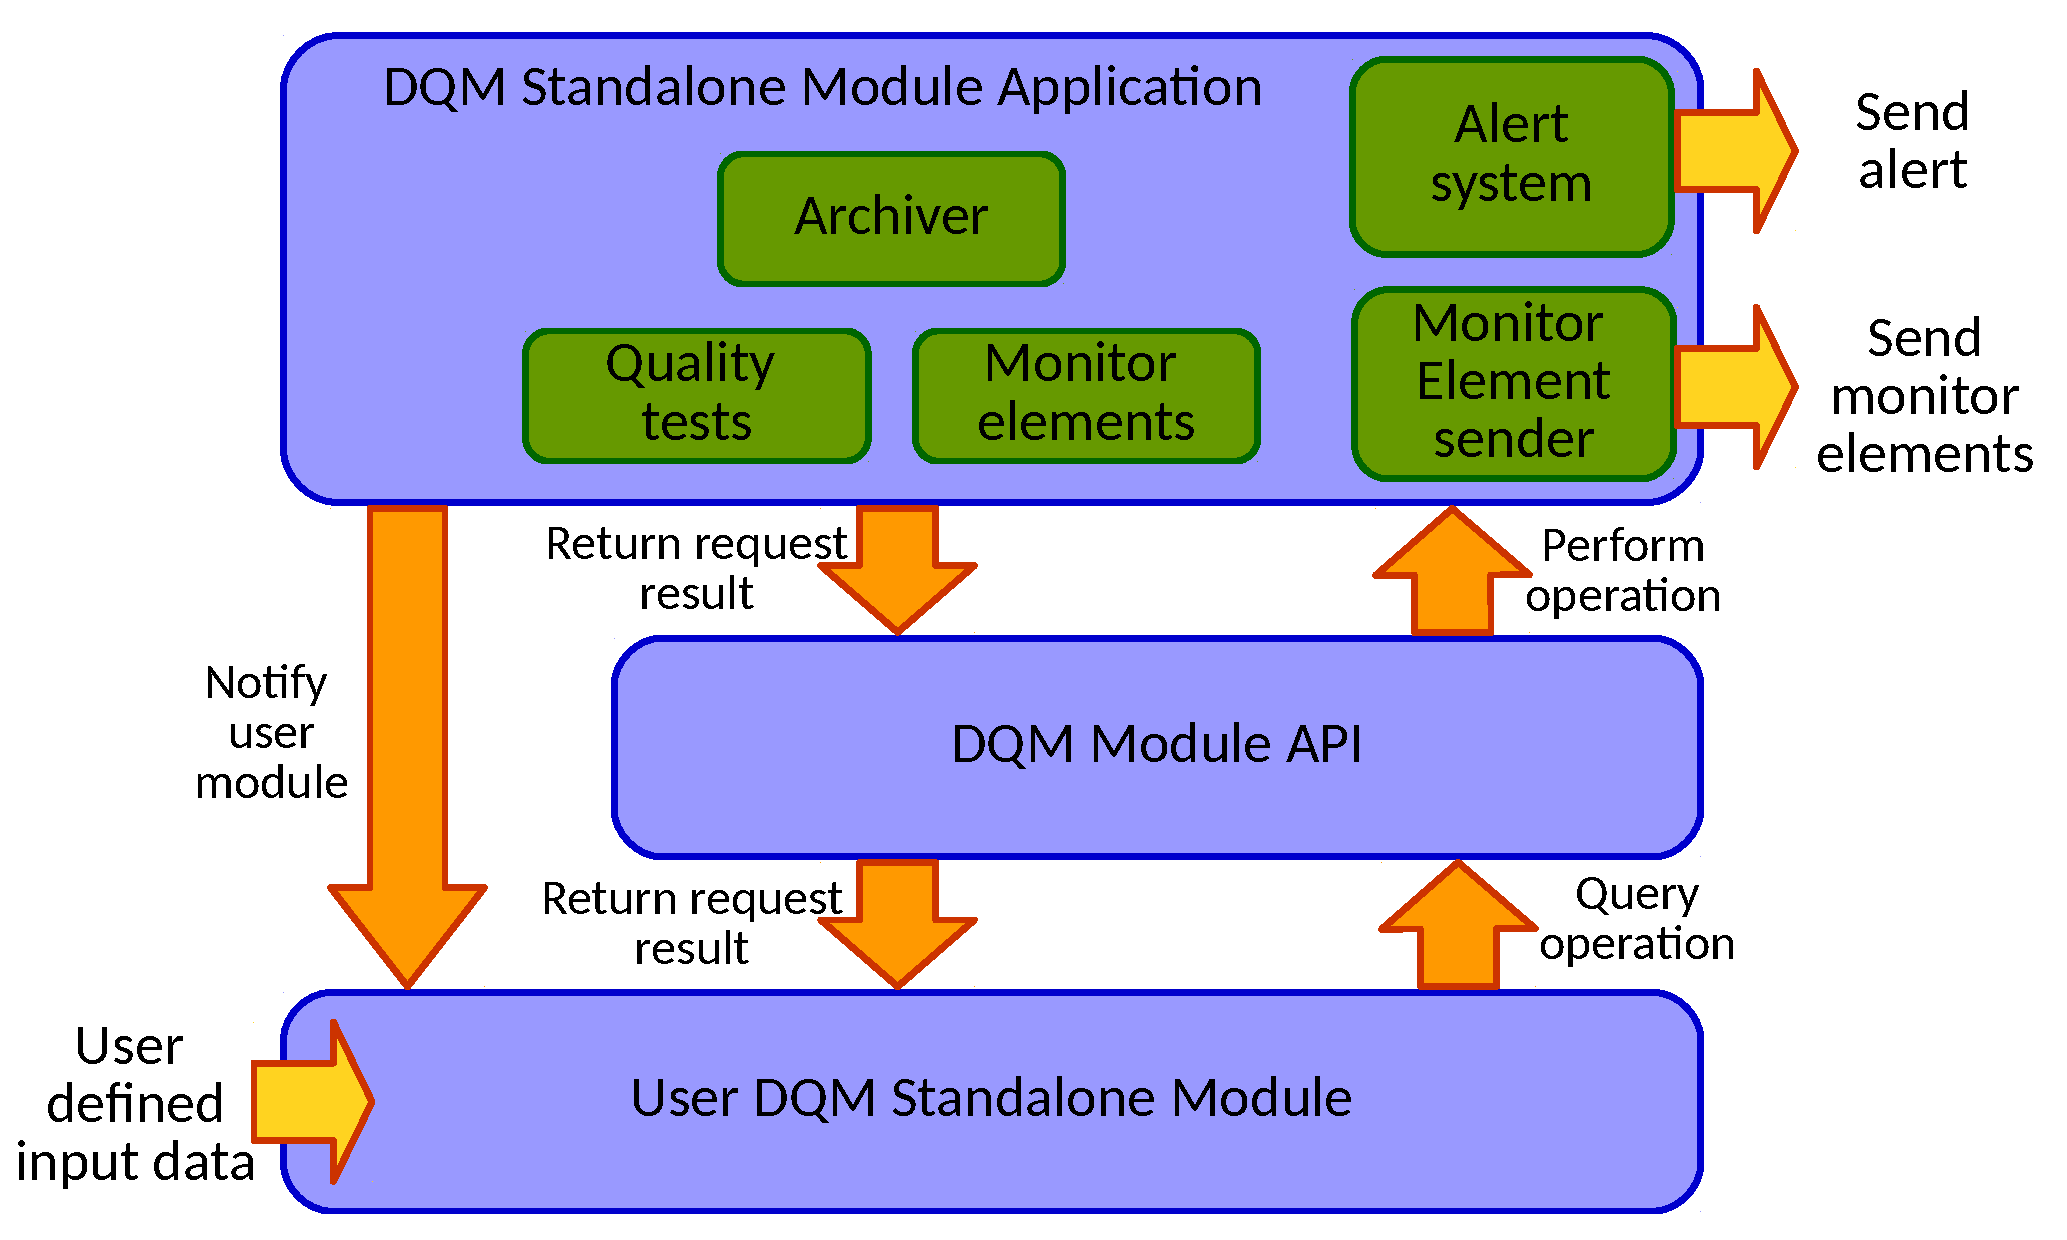
\includegraphics[width=0.9\linewidth]{figs/StandaloneModuleApplicationDiagram.pdf}
\end{frame}

%----------------------------------------------------------------------
\begin{frame}
  \frametitle{DQM4HEP}
  \framesubtitle{Online monitoring interface (Qt Gui)}
    \centering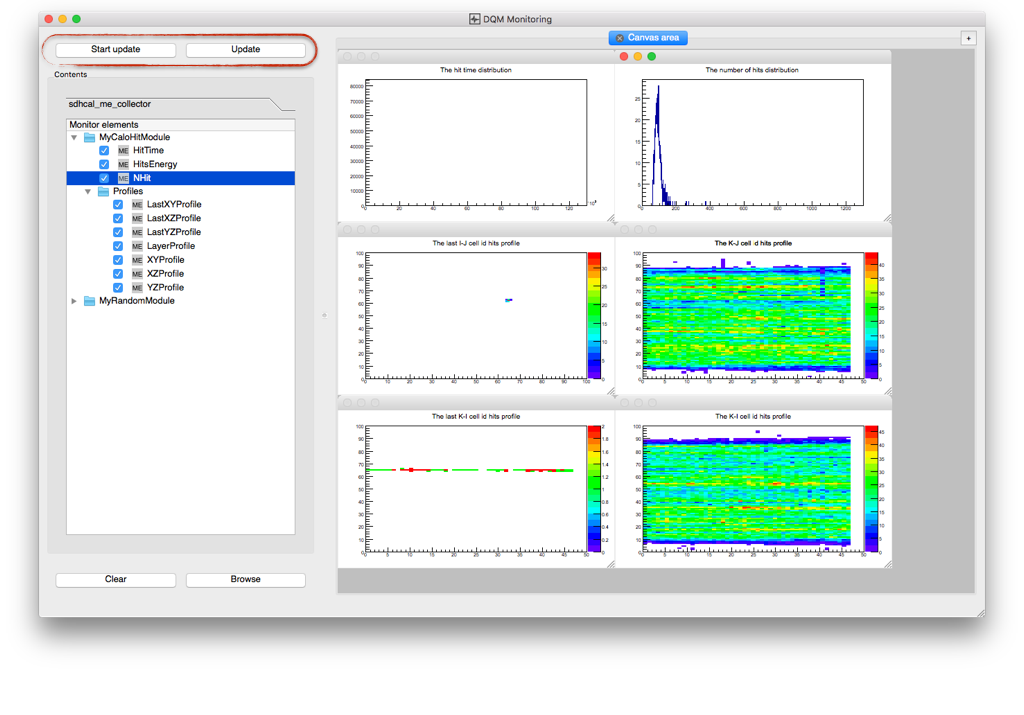
\includegraphics[width=0.95\linewidth]{figs/DQM4HEPMonitoringGui.png}
\end{frame}

%----------------------------------------------------------------------
\begin{frame}
  \frametitle{DQM4HEP}
  \framesubtitle{Detectors using DQM4HEP}
  DQM4HEP used by different detectors in the CALICE collaboration. \\
  ~\\
  
  \begin{minipage}{0.49\linewidth}
    SDHCal online monitoring
    \begin{itemize}
      \item Hit map
      \item Electronics rate
      \item Slow control : I, HV, LW, T, P
      \item GRPC efficiency, multiplicity
    \end{itemize}
    ~\\
    AHCal online monitoring
    \begin{itemize}
      \item Hit map
      \item Correlation with Telescope hits
      \item Electronics rate
    \end{itemize}
  \end{minipage}
  \begin{minipage}{0.49\linewidth}
    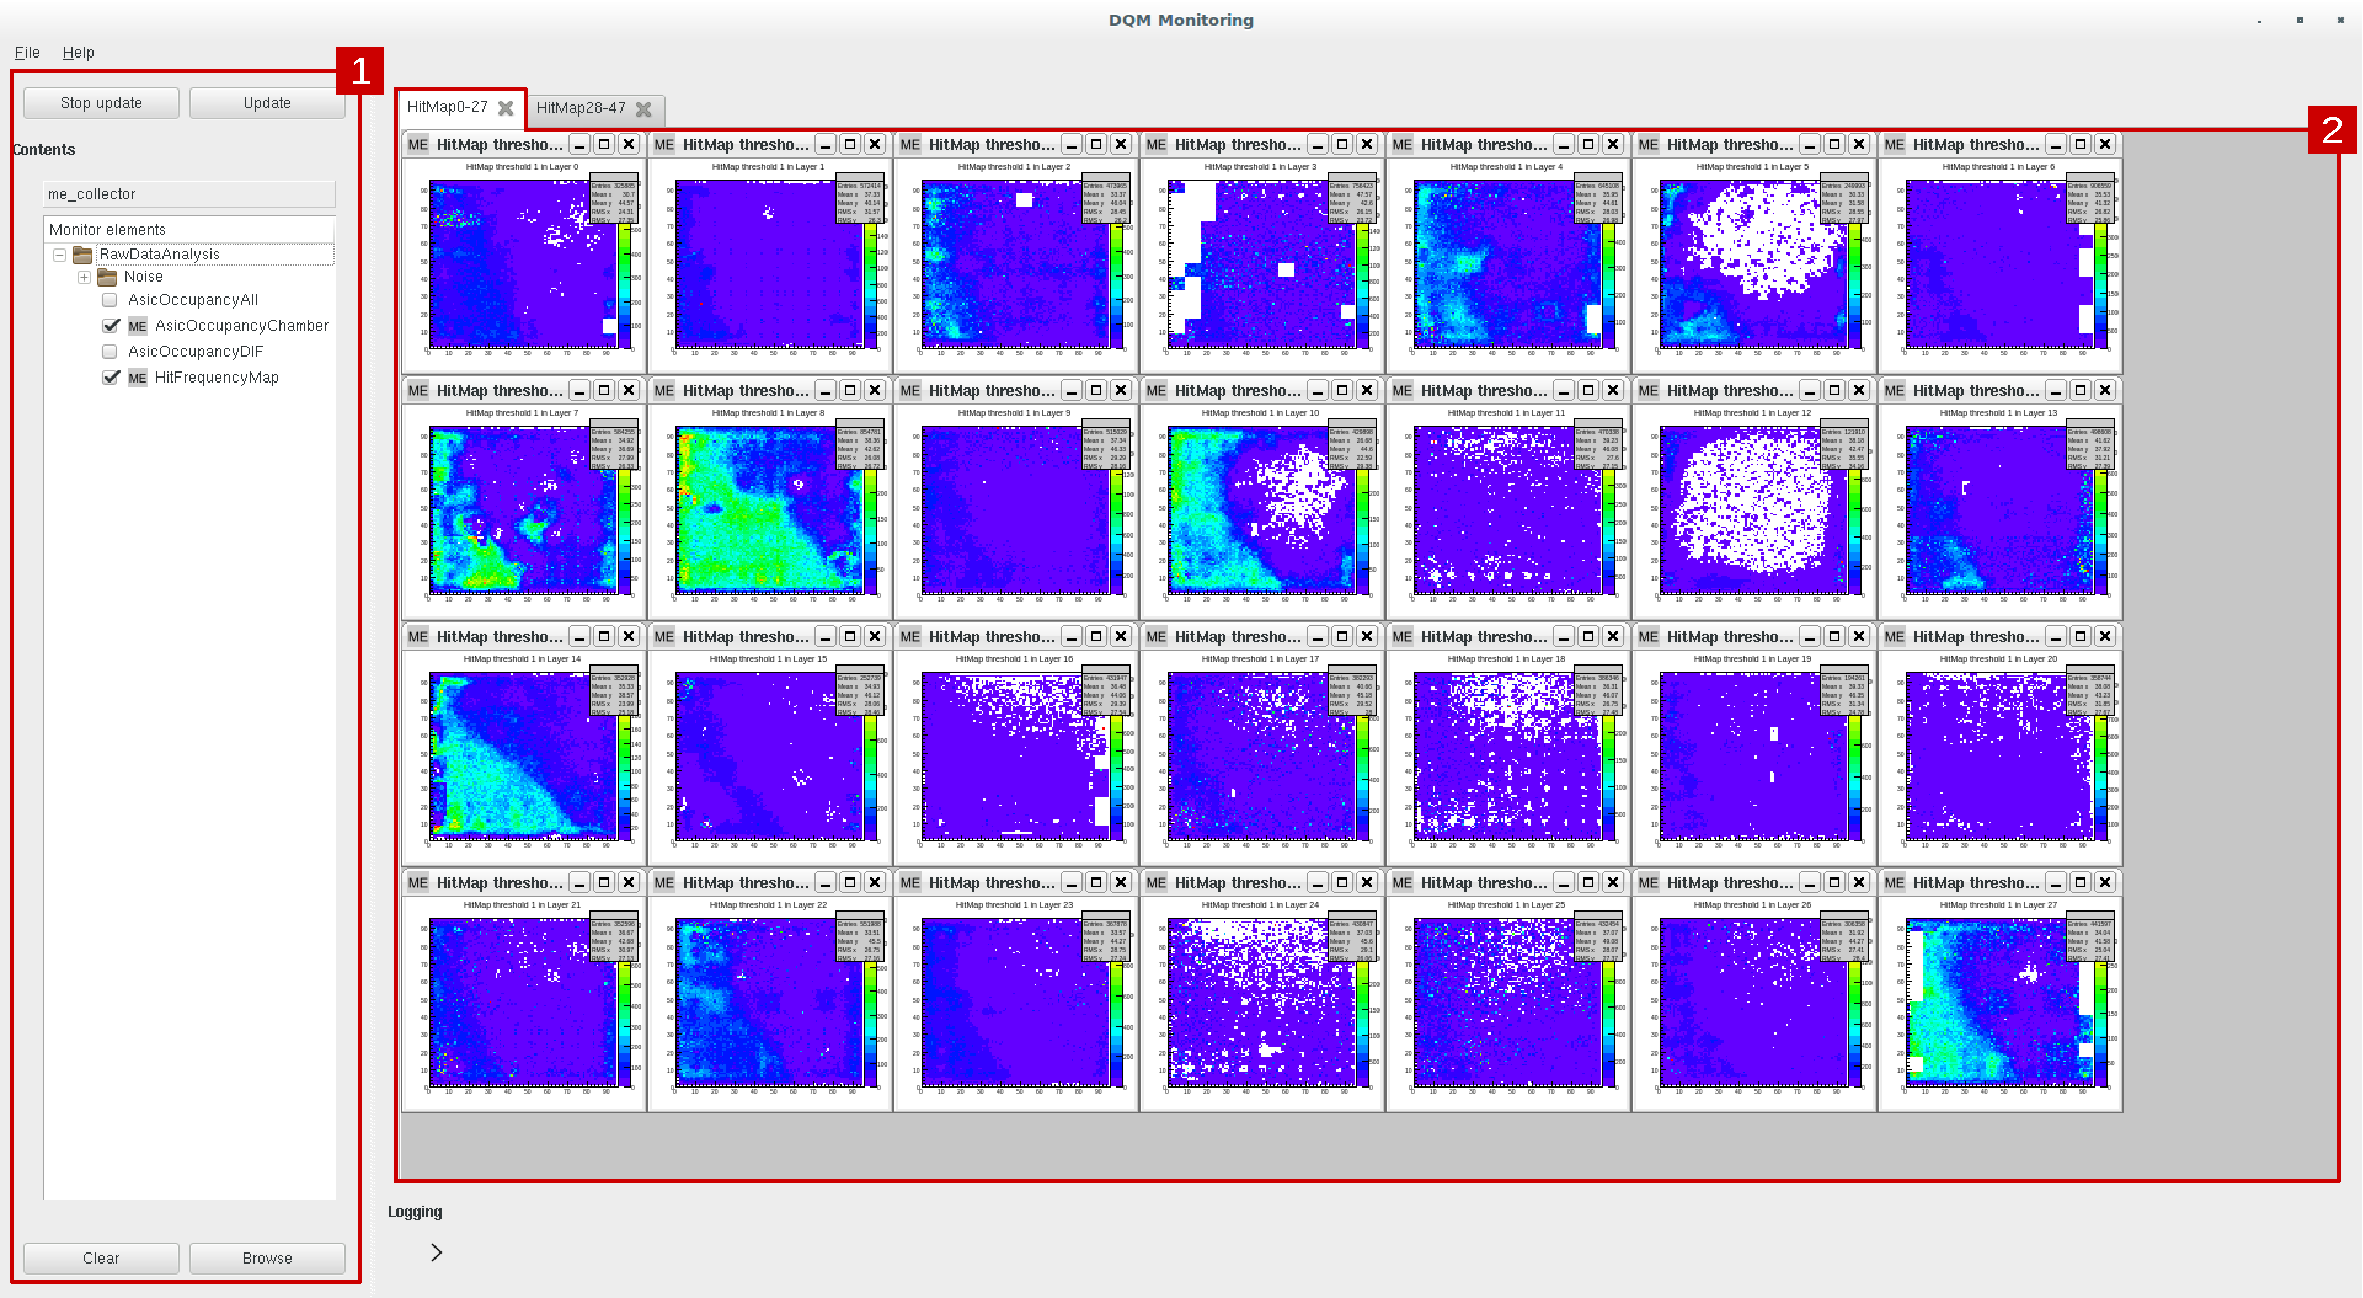
\includegraphics[width=0.95\linewidth]{figs/MonitoringMainWindowGui.pdf} \\
    ~\\
    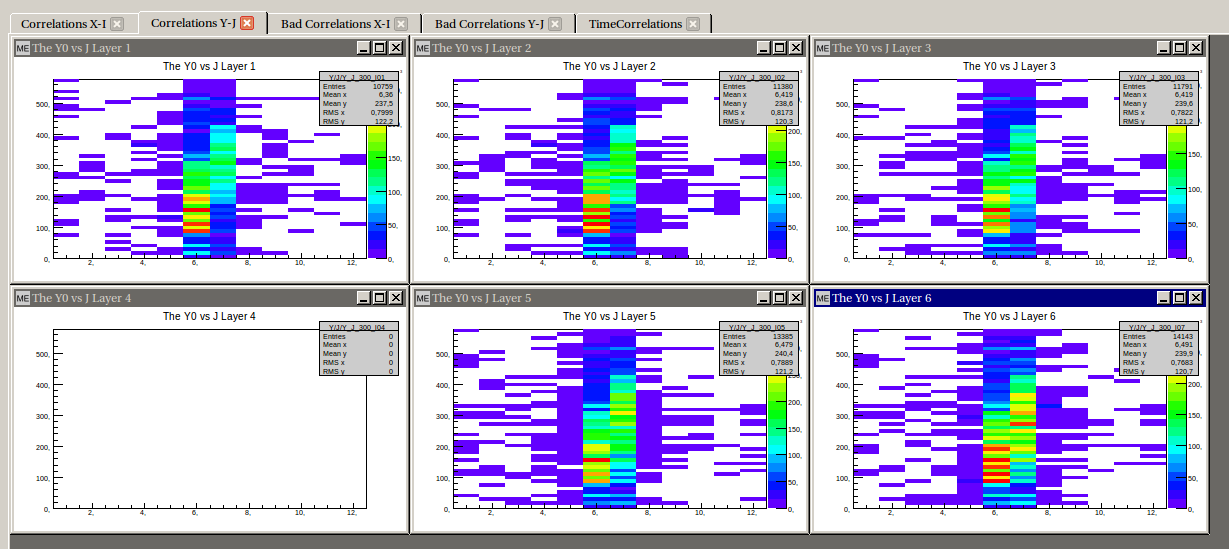
\includegraphics[width=0.95\linewidth]{figs/AHCal_DQM4HEP_CorrelationsYJ.png}
  \end{minipage}
\end{frame}


%----------------------------------------------------------------------
\begin{frame}
  \frametitle{DQM4HEP}
  \framesubtitle{AIDA2020 WP5 / WP15 }
  \scriptsize
  DQM4HEP developed within AIDA2020 WP5 (see MS67):
  \begin{center}
    \fbox{
      \begin{minipage}{0.5\linewidth}
        \begin{center}
          \textit{Task 5.4 Development of data quality \\
          and slow control monitoring}
        \end{center}
      \end{minipage}
    }
  \end{center}
  EUDAQ also developed within AIDA2020 WP5 as the DAQ solution (see MS46). \\
  ~\\
  Plan an \underline{integration in the EUDAQ event builder}
  \begin{itemize}
    \item Replace current EUDAQ monitoring
    \item Send event to DQM4HEP event collector before writing to disk
  \end{itemize}
  ~\\ 
  Once this is achieved, the two frameworks will provide a rather \textcolor{red}{complete and robust suite for test beam data taking}.\\
  ~\\
  DESY slow control monitoring developped within AIDA2020 WP15. \\
  ~\\
  Plan also for developing a DQM4HEP generic slow control module for the DESY test beam area, based on the SC software (see next talk by M. Wu).
\end{frame}


%----------------------------------------------------------------------
\begin{frame}
  \frametitle{DQM4HEP}
  \framesubtitle{Status - Ongoing work}
  \footnotesize
  \begin{itemize}
    \scriptsize
    \item Current available version is \texttt{v01-04-04}:
    \begin{itemize}
      \scriptsize
      \item Fully working version, used as proof of principle
      \item EUDAQ-DQM4HEP interface not feasable (run control)
      \item Module configuration (xml files) messy in case of a multiple host deployment
      \item No clear seperation between online and offline tools
      \item No documentation available for users ...
    \end{itemize}
    \pause
    \item Refactoring on-going:
    \begin{itemize}
      \scriptsize
      \item \textcolor{green}{\checkmark} Separation of the framework into Core / Net / Online / Vis packages
      \item \textcolor{green}{\checkmark} Make the classes more C++11 like and re-usable
      \item Necessary refactoring to allow for EUDAQ binding
      \begin{itemize}
        \scriptsize
        \item \textcolor{green}{\checkmark} Run control re-implemented 
      \end{itemize}
      \item \textcolor{green}{\checkmark} Core and Net packages have been fully re-implemented
      \item \textcolor{blue}{\ding{58}} Online package in development
      \item \textcolor{red}{\ding{55}} ~Vis package not yet re-implemented
    \end{itemize}
  \end{itemize}
  
\end{frame}




%----------------------------------------------------------------------
\begin{frame}
  \frametitle{DQM4HEP}
  \framesubtitle{Ongoing work - More functionalities and projects}
  \footnotesize
  \underline{Framework functionalities:}
  \begin{itemize}
    \scriptsize
    \item \textcolor{green}{\checkmark} Custom interface to any DAQ run control (SOR/EOR/Status)
    \item Quality assessement in offline mode:
    \begin{itemize}
      \scriptsize
      \item \textcolor{green}{\checkmark} Configure your quality tests in an xml file
      \item \textcolor{green}{\checkmark} Run them on a ROOT file and output results (\textcolor{green}{\checkmark} file \textcolor{green}{\checkmark}console \textcolor{red}{\ding{55}} db)
      \item \textcolor{blue}{\ding{58}} Strong effort to develop built-in qtests for users (extensible)
    \end{itemize}
    \item \textcolor{green}{\checkmark} Database config: XML parser allows to fetch parameters from MySQL db
    \item \textcolor{blue}{\ding{58}} Javascript interface: visualization and steering through web pages   
    \item Documentation
    \begin{itemize}
      \scriptsize
      \item \textcolor{blue}{\ding{58}} User documentation (manual) written in parallel of ongoing development
      \item \textcolor{green}{\checkmark} Technical documentation (doxygen) generated/pushed online when a PR is merged
    \end{itemize}
    \item \textcolor{green}{\checkmark} Travis CI added for all packages
  \end{itemize}
  \pause
  ~\\
  \underline{More projects:}
  \begin{itemize}
    \scriptsize
    \item Development of DESY slow control monitoring with DQM4HEP
    \begin{itemize}
      \scriptsize
      \item Can run continuousely and provide information to users at any time
    \end{itemize}
    \item DESY beam line uses EUDAQ $\rightarrow$ DQM4HEP will comes for free on DESY beam line
    \item Looking for integration in other experiments ...
  \end{itemize}
  \pause
  \centering \fbox{\textbf{Timescale for a new version: $\sim$ June 2018 !}}
  
\end{frame}



%----------------------------------------------------------------------
\begin{frame}
  \frametitle{DQM4HEP}
  \framesubtitle{URLs and contact}
  \footnotesize
  \underline{GitHub collaboration} (contributing, issues)\\
  \vspace*{0.1cm}
  ~~~
  \begin{minipage}{0.03\linewidth}
    
\includegraphics[width=\linewidth]{figs/github-logo.png}
  \end{minipage}
  \href{https://github.com/dqm4hep}{\tt https://github.com/dqm4hep} \\
  ~\\
  \underline{Installation package} (\texttt{v01-04-04}) \\
  \vspace*{0.1cm}
  ~~~
  \begin{minipage}{0.03\linewidth}
    
\includegraphics[width=\linewidth]{figs/github-logo.png}
  \end{minipage}
  \href{https://github.com/DQM4HEP/dqm4hep/releases/tag/v01-04-04}{\tt https://github.com/DQM4HEP/dqm4hep/releases/tag/v01-04-04} \\
  ~\\
  \underline{Slack channel} (Announcements, forum, management) \\
  \vspace*{0.1cm}
  ~~~
  \begin{minipage}{0.035\linewidth}
    
\includegraphics[width=\linewidth]{figs/slack-logo.png}
  \end{minipage}
  \href{https://dqm4hep.slack.com}{\tt https://dqm4hep.slack.com} \\
  ~\\
  \underline{Documentation} (ongoing, be patient !) \\
  \vspace*{0.1cm}
  ~~~
  \begin{minipage}{0.03\linewidth}
    
\includegraphics[width=\linewidth]{figs/rtd-logo.png}
  \end{minipage}
  \href{http://dqm4hep.readthedocs.io}{Read the docs : \tt http://dqm4hep.readthedocs.io} \\
  ~~~
  \begin{minipage}{0.03\linewidth}
    
\includegraphics[width=\linewidth]{figs/doxygen-logo.png}
  \end{minipage}
  \href{https://dqm4hep.github.io/dqm4hep-doxygen/}{Doxygen : \tt https://dqm4hep.github.io/dqm4hep-doxygen/} \\
  ~\\
  \underline{Contact us!}
  \begin{itemize}
    \item R. Ete (\href{mailto:remi.ete@desy.de}{\tt remi.ete@desy.de}) 
    \item A. Pingault (\href{mailto:antoine.pingault@ugent.be}{\tt antoine.pingault@ugent.be})
    \item T. Coates (\href{mailto:tc297@sussex.ac.uk}{\tt tc297@sussex.ac.uk})
  \end{itemize}

\end{frame}



\end{document}

